\BiChapter{实验现象及讨论}{exprise}
我们在MNIST数据集上分别实现了深度置信网络与卷积神经网络,使用深度置信网络训练得到的模型实现了98.72\% 的识别正确率,使用卷积神经网络实现了98.9\%的识别正确率。我们在CIFAR-10数据集上实现一个卷积神经网络,实现了62\%的正确率,此外,通过Caffe测试了由xxx提出的网络构型的学习效果,并将其与我们的网络学习效果进行对比。
\BiSection{数据集简介}
xMNIST与CIFAR-10是学术界两个重要的数据集,这两个数据集一般作为标准数据集而存在,每当人们提出一种新的算法,都会用这两个数据集做验证,下面我们将简单介绍这两个数据集。
\BiSubsection{MNIST}
xMNIST数据集是一个真实世界中采集的手写数字图像数据集\citeup{lecun2010mnist},它由NIST会议收集并持有,读者可到MNIST主页免费获取该数据集。这个数据集一共含有4个文件,分别存储训练数据、训练标签、测试数据、测试标签。文件以二进制文件形式存储,不过我们可以很容易编写一段小代码将其转换成图像。训练集共含有60000个样本,测试集含有10000个样本,这些样本收集自500位不同的人的手写字体。

\begin{figure}[!htbp]
\centering
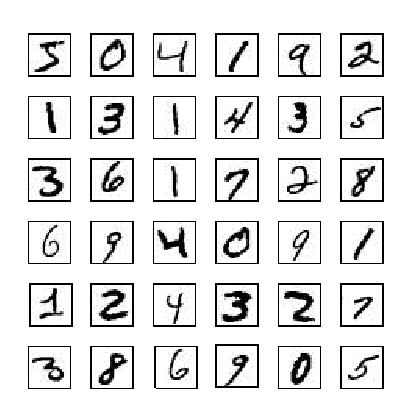
\includegraphics[width=0.3\textwidth]{expe/MNIST.eps}
\caption{MNIST数据集部分数据样本}
\label{img:MNIST data}
\end{figure}

每个数据样本是$28\times 28$像素的灰度图像,由于引入了抗锯齿效果,所以图像数值范围是$0\sim 255$而不是二值图像。图像已经经过预处理,因此图像会集中在中心$20\times 20$的区域内,此外,图像的中心点与像素点的重心重合,所以如果要使用模板匹配的方法(比如k近邻,SVM等)进行分类的话对图像再进行一些预处理使得数字的几何中心与图像中心重合会改善你的算法性能。



如图\ref{img:MNIST data}是MNIST数据集中的一小部分样本的展示,原始的数据应该是黑底白字的,为了美观,我们将其颜色反转并加上周围的边框。
\BiSubsection{CIFAR-10}
xCIFAR是一个由Alex Krizhevsky, Vinod Nair以及Geoffrey Hinton收集的一个含有8千万张图片的数据集\citeup{krizhevsky2009learningCIFAR},这些图片并没有经过手工标注。而CIFAR-10是这个数据集的一个子集,含有50000个训练样本和10000个测试样本,这些样本经过人手工标注为10个类别,分别是飞机、小汽车、鸟、猫等\citeup{alex2009cifar}。读者可以从CIFAR-10的官网免费获取这个数据集,它包含7个文件,其中有5个文件是训练集,每个文件包含10000个训练样本,有1个文件存储测试集,包含10000个样本,这些样本都被随机打散,所以不用担心类别的出现顺序会导致算法性能上的差异。剩余的一个文件是标签值与类别名字的键值对。CIFAR-10为我们提供了三种存储形式,分别对应Python、MATLAB与二进制形式的数据存储格式,读者可根据自己的语言背景选取其中一种进行下载。

\begin{figure}[!htbp]
\centering
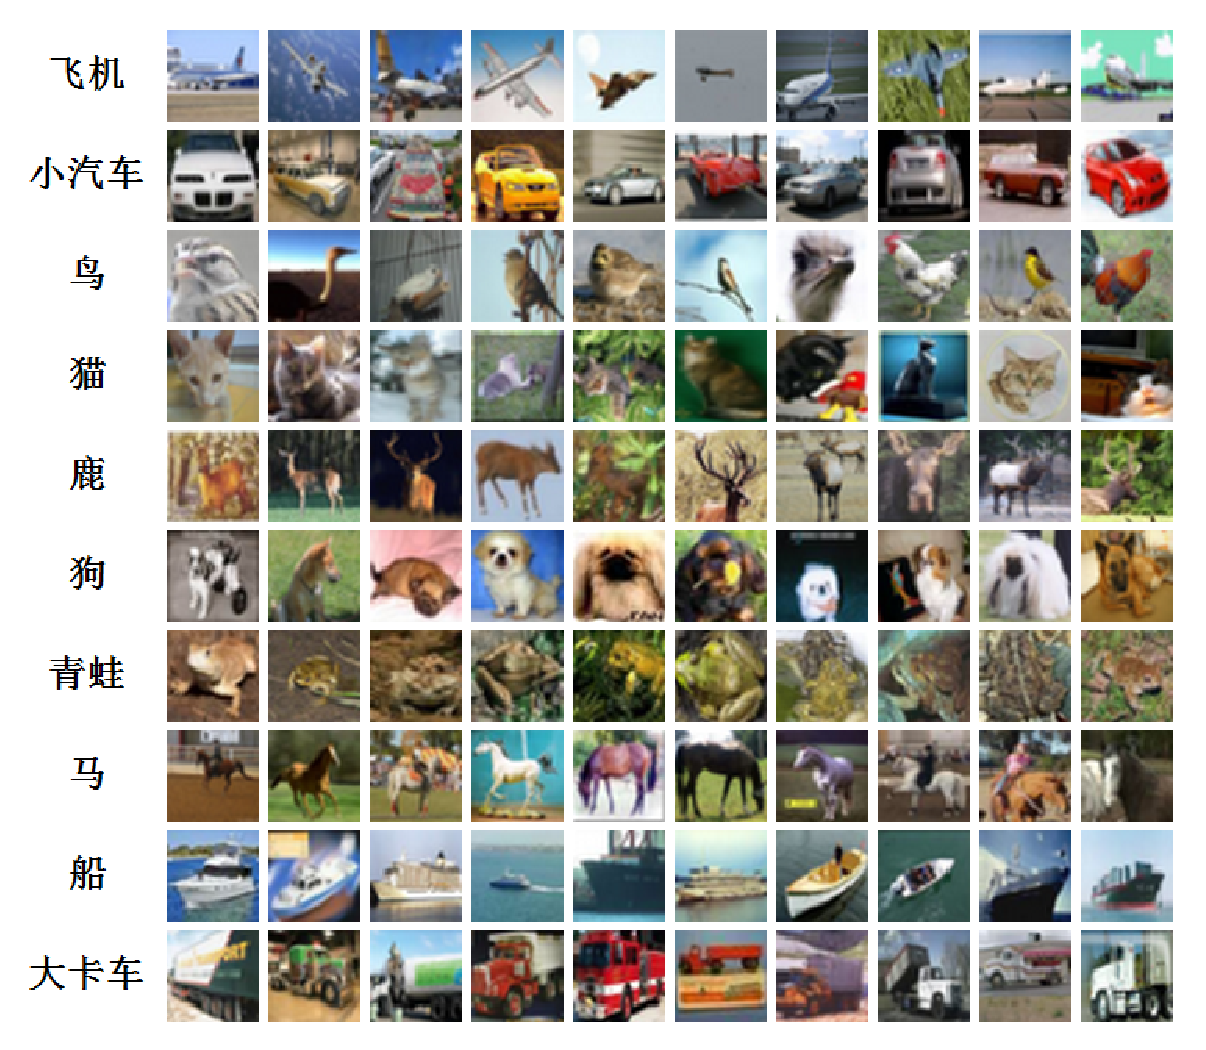
\includegraphics[width=0.6\textwidth]{expe/CIFAR-10.eps}
\caption{CIFAR-10数据集部分数据样本}
\label{img:CIFAR data}
\end{figure}

每个数据样本都是大小为$32\times 32$的彩色图像,因此每张图像应包含三张$32\times 32$大小的矩阵,分别代表R、G、B三个原色通道。如图\ref{img:CIFAR data}所示是这个数据集的一部分样本,我们可以看到,这些图像更接近于真实生活中的图像,相比于MNIST而言,每个类别个体的图像差异较大,而不像MNIST中每个类别的个体差异较小,所以在CIFAR-10数据集中使用模板匹配的方法进行分类是几乎不可能的。

\BiSection{深度置信网络在MNIST数据集上的性能}
x在MNIST数据集上,我们设计了一个7层神经网络,每层所含的节点分别是784、621、982、600、410、569、10,最底层的节点数是根据原始数据输入维度决定的,即$28\times 28 = 784$,最顶层的节点数是根据最终的类别决定的,即10个类别。中间的隐含层节点我们随意选取,这些节点是如此的随意以至于源自我的银行卡号。在深度置信网络中,对隐含节点并没有过多的要求,大致合理即可。

整个网络可以看做5个受限玻尔兹曼机叠加组成,分别是784$\sim$621,621$\sim$982,$\cdots$,410$\sim$569,最后一层569$\sim$10是softmax分类器。在整个网络的训练过程中,我们先依次对其中的5个受限玻尔兹曼机做贪婪训练,即先训练784$\sim$621的受限玻尔兹曼机,训练完毕后将所有的样本(60000个)通过这个训练完毕的受限玻尔兹曼机前向传播,得到60000个621维的数据样本,用这些维度变换后的样本训练下一个,即621$\sim$982的受限玻尔兹曼机,以此类推。最后的softmax分类器其预训练是将其当做一个两层softmax网络进行预训练。

观察受限玻尔兹曼机的权值更新公式\eqref{equ:MAMAMA}、\eqref{equ:MBMBMB}以及\eqref{equ:MCMCMC},为了方便大家观察,我们将这三个公式再一次书写一次

\begin{equation}
\frac{\partial\ln P(v)}{\partial w_{i, j}} \approx
 P(h_i = 1 | v^{(0)})v_j^{(0)} - P(h_i = 1 | v^{(k)})v_j^{(k)}
\end{equation}

\begin{equation}
\frac{\partial\ln P(v)}{\partial b_{vi}} \approx
v_j^{(0)} - v_j^{(k)}
\end{equation}

\begin{equation}
\frac{\partial\ln P(v)}{\partial b_{i}} \approx
 P(h_i = 1 | v^{(0)}) - P(h_i = 1 | v^{(k)})
\end{equation}

这三个公式背后隐藏着一层重构的含义,即对于一个两层的受限玻尔兹曼机,在第一层的数据通过前向传播得到第二层的数据,第二层的数据反向注入得到第一层的数据,数据经过这样一个迁移,相当于利用提取的特征重构原始样本,因此在受限玻尔兹曼机的训练过程中,一个刻画其训练情况的方法是跟踪其重构误差,如图\ref{img:Reconstruct Error des}所示是某一层受限玻尔兹曼机的重构误差下降曲线。

\begin{figure}[!htbp]
\centering
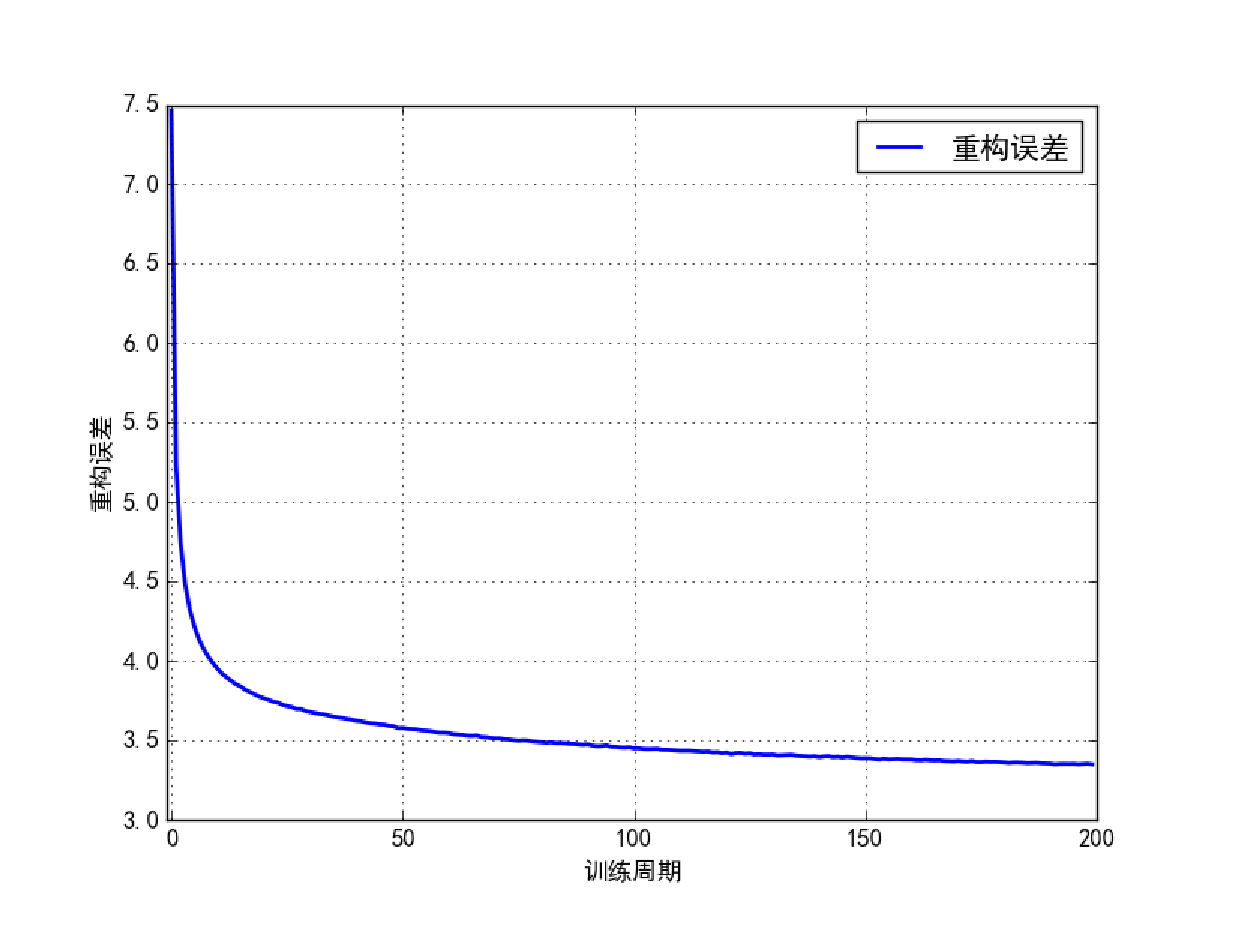
\includegraphics[width=0.5\textwidth]{expe/RBMReconstructError.eps}
\caption{受限玻尔兹曼机重构误差下降曲线}
\label{img:Reconstruct Error des}
\end{figure}

从图\ref{img:Reconstruct Error des}中我们不难发现,训练的前10个周期重构误差迅速下降,随后的周期下降速度缓慢,因此如果你的实验时间有限,那么可以只训练较少的周期即可,但训练更多的周期会有助于获取更好的实验结果。需要提到的一点是,在受限玻尔兹曼机的训练中,动量项是必须的,我们在实验中发现,不使用动量项时,在训练的初始阶段重构误差无法下降。

我们还追踪了受限玻尔兹曼机对图像的具体重构,如图\ref{img:Reconstruct Number}所示是一些样本在784$\sim$621的受限玻尔兹曼机中的重构情况,原始样本与重构样本我们已在图中标注。需要提醒的是,图\ref{img:Reconstruct Number}中的原始图像与图\ref{img:MNIST data}中的原始图像不一致,这是因为图\ref{img:MNIST data}中的样本每个像素点取值是$0\sim255$,而我们将这些像素点$01$化,所使用的方法是,对每个像素点除以255得到一个[0,1]区间的小数$p$,以数值$p$为概率将其置1,以$1-p$为概率将其置0。另一种01化的方法是,直接保留这个小数而不将其离散化。

\begin{figure}[!htbp]
\centering
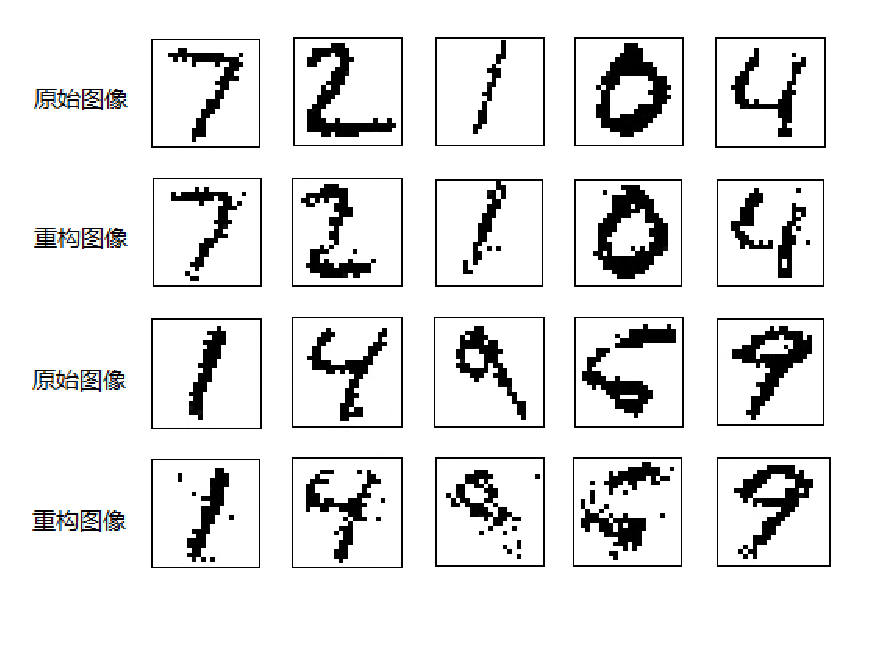
\includegraphics[width=0.4\textwidth]{expe/reconstructImage.eps}
\caption{受限玻尔兹曼机对数字的重构}
\label{img:Reconstruct Number}
\end{figure}

最顶层的softmax分类器的训练也是贪婪的,即它只训练569$\sim$10两层网络之间的参数,在这里,训练周期我们不建议太长,一般训练5$\sim$10个周期即可,否则在随后的方向传播过程中,如果softmax预训练过久,则网络的输出误差较小,没有误差就难以进行反向传播,全局微调容易失败,这会导致网络陷入局部最优解,这个局部最优由最顶层的softmax决定而不是整个网络决定。

当整个网络预训练完毕后,我们执行全局的反向传播算法对参数进行微调,这个过程与传统的神经网络相同,我们不进行过多的叙述,如图\ref{img:DBN Error des}所示是整个网络进行反向传播时的误差下降曲线

\begin{figure}[!htbp]
\centering
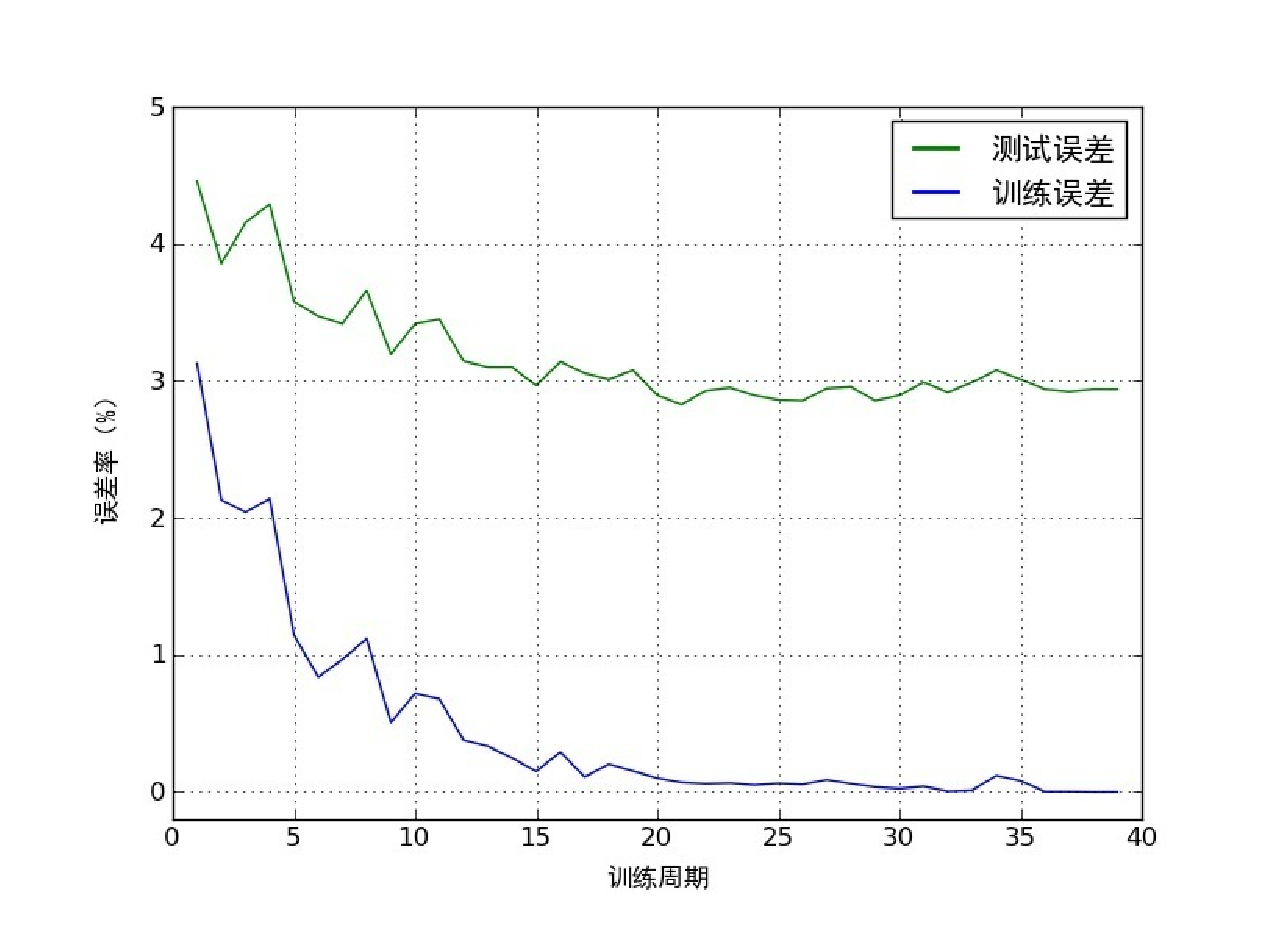
\includegraphics[width=0.5\textwidth]{expe/DBNTrainingErrorAndTestError.eps}
\caption{深度置信网络误差下降曲线}
\label{img:DBN Error des}
\end{figure}

细心的读者会发现,图\ref{img:DBN Error des}的下降曲线表明最终这个网络并没有收敛到我们号称的正确率98.72\%,确实如此,因为我们在数据迁移时遗失了一部分的数据,图\ref{img:DBN Error des}中的数据是前期研究工作中没有遗失的数据,因此这并不是最终的误差下降曲线。但是我们的实验是可重现的,只需按照我们的结构便可再现98.72\% 的正确率,由于我们的时间有限,并没有将这个实验重新做一遍,感兴趣的读者可以尝试。

网络训练完毕后,我们选取了一部分网络识别错误的数字,将其展示在图\ref{img:errorClassify}中,每个样本下边的黑色数字代表测试集给定的标签,而红色数字代表网络的预测标签。我们可以发现,这些错误的样本中,有一部分自身就带有二义性,人也难以区分究竟是哪个数字,而有一部分样本人可以很容易识别,网络却识别错误,还有一部分样本数据本来就是错误的,根本无法识别它是哪个数字,这时候我们不能舍弃机器也能将其识别出来。

\begin{figure}[!htbp]
\centering
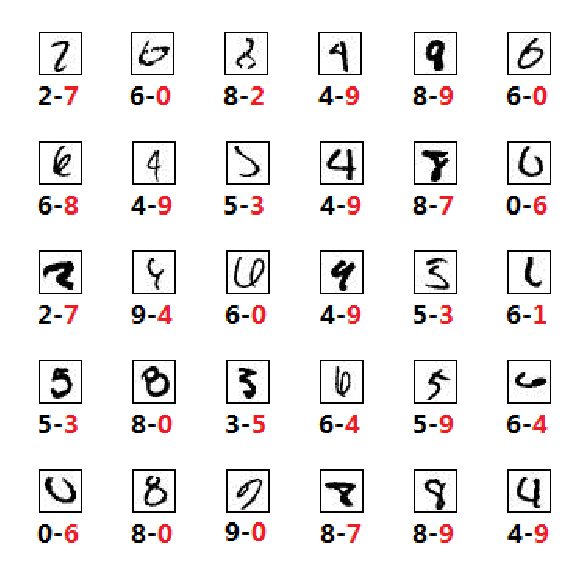
\includegraphics[width=0.4\textwidth]{expe/errorClassify.eps}
\caption{被网络误分类的样本}
\label{img:errorClassify}
\end{figure}

在整个网络的训练中,我们使用了动量项、权衰减技术,而没有没有使用降维技术,因为数据维度并不是特别高,计算机的处理能力足以应付。如果原始数据的维度非常高,比如几百万维,那么就需要采用一些降维技术将原始数据进行压缩。

深度置信网络在一定程度上仍然带有模板匹配的气息,因为我们如果只使用2000个样本作为训练集而不是全部的60000个样本,网络也能实现90多的正确率,后面中的实验中我们会看到,这种策略在卷积神经网络中是行不通的。


\BiSection{卷积神经网络在MNIST数据集上的性能}
x在MNIST数据集,我们设计了一个6层卷积网络,其网络构型描述如下
\begin{itemize}
\item 1张$28\times 28$的原始图像
\item 卷积原始图像得到6张$24\times 24$特征图
\item 对6张特征图进行采样得到6张$12\times 12$特征图
\item 对6张特征图进行卷积得到12张$8\times 8$特征图
\item 对12张特征图进行采样得到12张$4\times 4$特征图
\item 此时12张$4\times 4$特征图无法再进行卷积,将其展开得到192个节点
\item 192个节点与10个输出节点做全连接网络,与传统神经网络一样
\end{itemize}

其中,激活函数我们选取的是sigmoid函数,当然这个函数也可以换成ReLU函数,全连接网络我们采用平方误差作为准则,而不是深度置信网络中的softmax分类器。在这个网络中,我们不采用预训练而是直接进行全局的反向传播。以上的网络构型的选取方案都是随意的,并没有说一定要采用这个方案。

实验获取的训练误差及测试误差曲线如图\ref{img:CNNTrainingErrorAndTestError}所示,训练完毕后,我们在MNIST上取得了98.9\%的正确率。我们可以看到,在网络训练的前20个周期,训练误差与测试误差迅速下降,随后的周期中误差缓慢下降,到了后期,收敛十分缓慢,但依然会有下降的趋势。有意思的是,对网络训练一个很长的周期并不会产生明显的过学习现象,所以如果你需要实现一个高识别率的网络,那么你可以放心地等待一段很长的的时间。

值得注意的是,误差下降过程带有明显的波动性,在深度置信网络的训练过程中,一般到了训练的后期,识别率不会有太大的波动,比如,深度置信网络在到达98.70\%的正确率后,其波动范围就在98.70\%附近波动,可能是98.73\%、98.74\%。然而,在卷积网络中,到达98.70\%后,它可能一下子跌到98.40\%,然后又升到98.80\%,这种较大范围的波动,应该不是随机梯度造成的,因为深度置信网络中我们采取随机梯度更新时也没有这么大的波动,我们推测这是因为卷积网络代表着一种非常强的惩罚(强迫权值共享),惩罚过大导致波动变大。

\begin{figure}[!htbp]
\centering
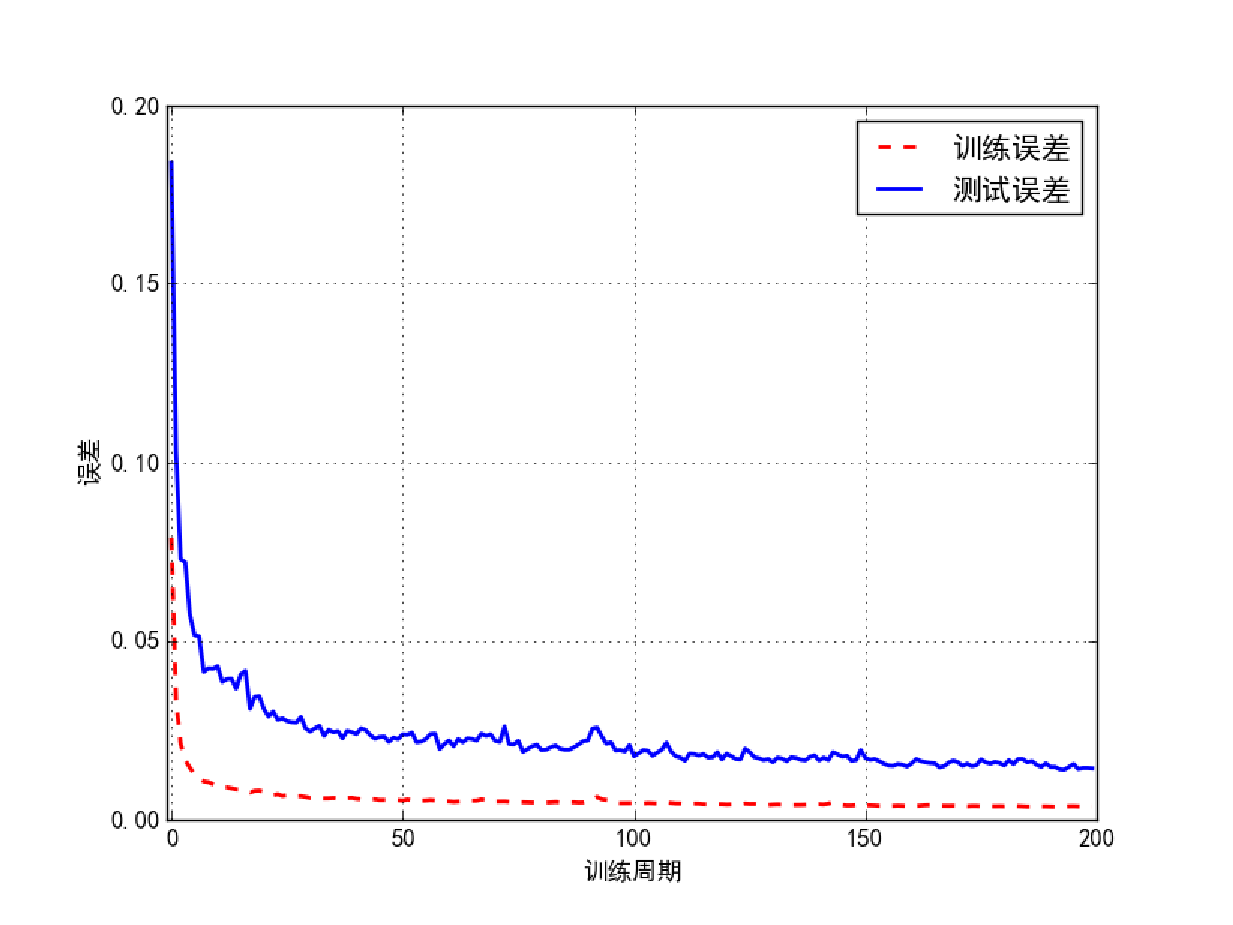
\includegraphics[width=0.5\textwidth]{expe/CNNTrainingErrorAndTestError.eps}
\caption{卷积神经网络训练误差及测试误差}
\label{img:CNNTrainingErrorAndTestError}
\end{figure}

在实验中,我们并没有采用权衰减,因为我们发现使用权衰减后网络的性能变差。此外,我们发现当改变网络中的一些参数,比如特征图的张数,学习率时,对网络的收敛影响较大,但对最终结果并没有太大影响。卷积网络对样本的需求量非常大,实验中,我们选取2000个样本作为训练集对网络进行训练,网络完全不会收敛,这与深度置信网络是不一样的,只有我们将所有的60000个样本作为训练集对网络进行训练时,网络才开始收敛。我们估计这是因为卷积网络的权值共享导致它只有通过大量的样本才能学习特征,这与模板匹配方法有着很大的区别。

网络训练完毕后,我们对测试集中的一部分数据进行观察,第一层卷积层提取出的特征如图\ref{img:CNNFeatureMaps}所示。我们分别选取了$0\sim 9$一共10个样本,每一行代表一个样本。其中,每一行的第一张是原始的$28\times 28$图像,随后六张是卷积出来的六张$24\times 24$大小的特征图。观察图\ref{img:CNNFeatureMaps},我们可以发现一些有意思的现象。例如,原始图像是黑底白字的,而有一些特征图反转成为白底黑字,又比如,第六张特征图是对图像进行边界检测,为了验证我们这个想法,我们随机选取了“4”这个数字的几个样本进行特征抽取,其结果如图\ref{img:fourNumber} 显示,通过观察,我们不难发现,对于不同的写法,其提取到的特征都是近似的,它会检测“4”的左边竖线的上方一点以及对下来的一个折线,右边竖线的上方一点以及下方的一点。另一个有意思的现象是,第三张特征图看起来是一个3D图像,想象图像的左上角有一束阳光洒下,当我们伸出右手,掌心贴着当前的纸张页面,大拇指朝纸张左方,握拳,数字经过我们四个手指的方向旋转过一定角度后,那么阳光洒下的阴影如同第三张特征图所示。这个现象在第五张特征图中也出现了,只是第五张特征图的阳光处于左侧而不是左上角。同样伸出我们的右手,掌心贴着当前的纸张页面,大拇指朝纸张下方,握拳,我们可以看到数字经过我们四个手指的方向旋转过一定角度后,阳光洒下的投影正如第五张特征图所示。

\begin{figure}[htbp]
\centering
\subfigure{\label{img:CNNFeatureMaps}}\addtocounter{subfigure}{-2}
\subfigure{\subfigure[针对0-9不同数字提取到的特征图像]
			{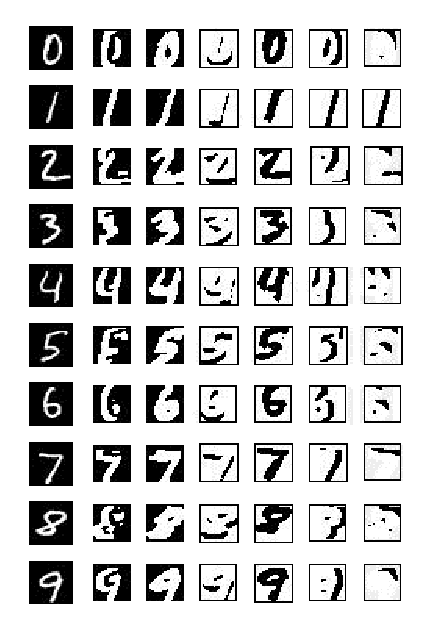
\includegraphics[width=0.4\textwidth]{expe/CNNFeatureMaps.eps}}}
\subfigure{\label{img:fourNumber}}\addtocounter{subfigure}{-2}
\subfigure{\subfigure[针对数字“4”提取到的特征]
			{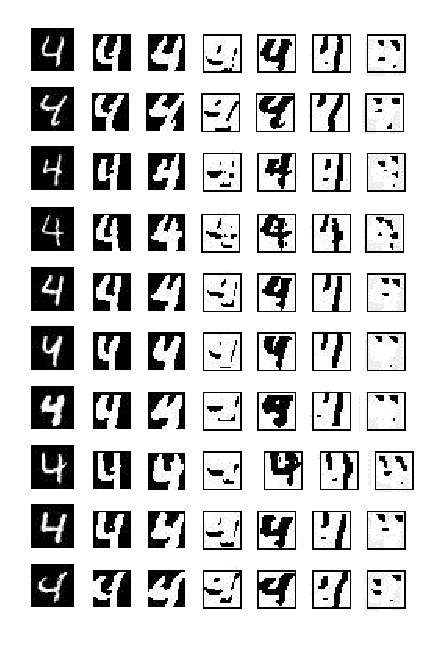
\includegraphics[width=0.405\textwidth]{expe/fourNumber.eps}}}
\caption{第一层卷积层抽取得到的特征图}
\label{img:CNNferture}
\vspace{-1em}
\end{figure}



\BiSection{卷积神经网络在CIFAR-10数据集上的性能}
x相比于MNIST数据集,CIFAR-10数据集的识别更为困难。由于计算资源的限制,我们只在CIFAR-10上设计了一个较小的卷积网络,与MNIST手写数字的卷积网络构型类似,在CIFAR-10数据集上,我们同样设计了一个4层卷积网络,其网络构型描述如下
\begin{itemize}
\item 3张$32\times 32$的原始图像
\item 卷积原始图像得到9张$28\times 28$特征图
\item 对9张特征图进行采样得到9张$14\times 14$特征图
\item 尽管9张$5\times 5$特征图仍然可以被卷积,但我们依然将其展开为1764个节点
\item 1764个节点与10个输出节点做全连接网络,与传统神经网络一样
\end{itemize}

网络的属性与MNIST实验中的相同,激活函数我们依然选取sigmoid函数,全连接网络依然采用平方误差作为准则,对网络进行训练得到训练集误差下降如图\ref{img:CIFAR train error }所示,测试集误差量下降如图\ref{img:CIFAR test error}所示。需要注意的是,看起来在图\ref{img:CIFAR train error }与图\ref{img:CIFAR test error}中误差下降速度非常快,对比与图\ref{img:CNNTrainingErrorAndTestError},其斜率更大,然而这是一个假象,因为我们对纵轴进行了尺度缩放,事实上在CIFAR中误差下降的非常慢,而且在训练集与测试集中仍然后很大的误差可以下降。

\begin{figure}[htbp]
\centering
\subfigure{\label{img:CIFAR train error }}\addtocounter{subfigure}{-2}
\subfigure{\subfigure[训练误差下降曲线]
			{\includegraphics[width=0.45\textwidth]{expe/CIFARtrainError.eps}}}
\subfigure{\label{img:CIFAR test error}}\addtocounter{subfigure}{-2}
\subfigure{\subfigure[测试误差下降曲线]
			{\includegraphics[width=0.45\textwidth]{expe/CIFARtestError.eps}}}
\caption{CIFAR的训练误差与测试误差}
\vspace{-1em}
\end{figure}

因为CIFAR-10数据集的复杂性,本应该建立一个庞大的网络进行训练,但由于我们的计算资源有限,时间紧迫,所以无法实现一个更大的卷积网络,此外,对网络的训练我们也仅仅训练了400个周期左右,因此,整个网络训练完毕后我们只得到62\%的识别正确率。

如图\ref{img:CIFARcorrectClassfy}所示是一部分被网络正确识别的样本,其中每一行代表一个类别,图中总共包含了10个类别100个样本。观察这些样本我们会发现,网络能识别的图像对位移、旋转等性质具有不敏感性。例如,在飞机这个类别中,网络可以识别头部向左、向右等多个角度的飞机,还可以识别俯仰角不同的图片,由于这些图片不具备模板性,所以卷积网络基本没有了模板匹配的缺点。

\begin{figure}[!htbp]
\centering
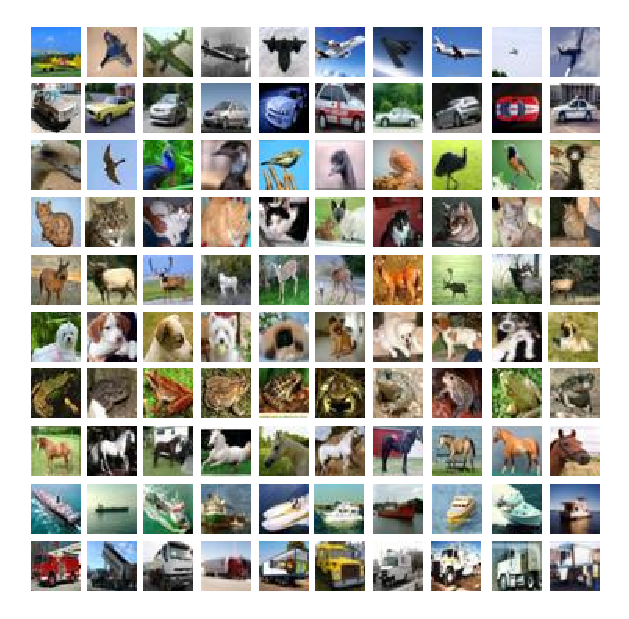
\includegraphics[width=0.6\textwidth]{expe/CIFARcorrectClassfy.eps}
\caption{被网络正确识别的CIFAR-10部分样本}
\label{img:CIFARcorrectClassfy}
\end{figure}

我们跟踪了网络无法识别的样本,将其一部分绘制如图\ref{img:CIFARerrorClassfy}所示。图中每个样本下方的黑色数字代表由训练集提供的标签值,而红色数字代表网络的输出标签值,标签值于类别名字的键值对可参照图\ref{img:MNIST data}。我们发现,在一些样本中,网络会将大卡车错误地识别成小汽车或将小汽车错误地识别成大卡车,这似乎可以原谅,但有一些图像的错误识别是我们无法原谅的,例如将马识别成大卡车。这些错误的样本中很多样本人是可识别的,而机器不可识别,我们推测这是因为我们的网络设计得不够庞大,训练周期也步长,导致网络无法进行更好的特征提取,从而影响最终的识别效果。

\begin{figure}[!htbp]
\centering
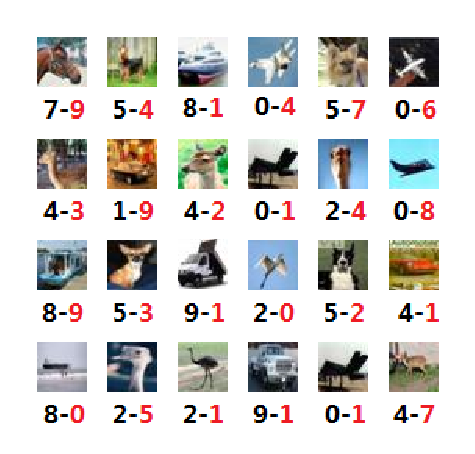
\includegraphics[width=0.4\textwidth]{expe/CIFARerrorClassfy.eps}
\caption{被网络错误识别的CIFAR-10部分样本}
\label{img:CIFARerrorClassfy}
\end{figure}

为了描述网络的特征提取性能,如同在MNIST上卷积网络的工作,我们同样将第一层卷积层提取到的特征绘制如图\ref{img:CIFARfeatureMap}所示。我们选取了“飞机”类别下的9个样本,每一行代表一个样本。其中,每一行的前三张黑白图像是原始$32\times 32$大小的RGB通道,这三张图像合成第四张$32\times 32$彩色图像。随后的九张是第一层卷积层提取到的九张$28\times 28$大小的特征图。对比这些原始数据与特征图,我们发现,原始数据中图像是含有冗余的,大部分的特征图过滤掉这些冗余信息,将飞机的边界提取出来形成特征图。这些特征图中,有一些特征例如第2张,第8张并没有提取到一些人可理解的特征,我们猜测随着训练周期的增加,这些特征将会逐渐显露出来,由于时间有限,我们并没有验证我们的猜想。


\begin{figure}[!htbp]
\centering
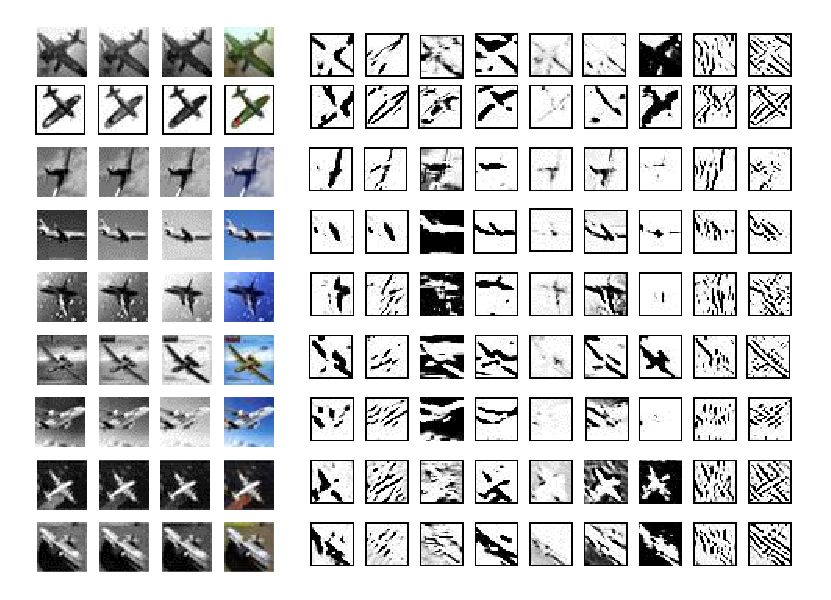
\includegraphics[width=0.8\textwidth]{expe/CIFARfeatureMap.eps}
\caption{针对“飞机”类别提取的特征}
\label{img:CIFARfeatureMap}
\end{figure}

这些特征图应该可以通过选取某几张组成彩色的特征图,但我们并不知道选取哪几张合适,所以我们并没有做这一步工作。此外,这些特征图表明,在他们之上应该再添加一些卷积层对特征继续提取,而不是我们设计的全连接网络,由于我们的计算资源十分匮乏,所以我们也没有进一步展开这项工作。

\BiSection{使用Caffe实现的CIFAR-10数据集训练}
x目前学术界认为CIFAR-10数据集已被解决,因为最好的识别效果由xxx实现,正确率为91\%。另一识别率较高的网络由Alex Krizhevsky等人实现,其识别率为89\%,这个网络稍微有点复杂所以我们不会在本文中提及,更多的讨论可阅读其论文xxxx。在Caffe中的卷积网络构型采取的是Alex Krizhevsky的方案,为了实现对比,我们使用Caffe验证了Alex Krizhevsky等人的网络构型在CIFAR-10数据集上的训练效果,其训练误差与测试误差曲线如图\ref{img:caffeError}所示

\begin{figure}[htbp]
\centering
\subfigure{}\addtocounter{subfigure}{-2}
\subfigure{\subfigure[训练误差下降曲线]
			{\includegraphics[width=0.45\textwidth]{expe/caffeTrainErr.eps}}}
\subfigure{}\addtocounter{subfigure}{-2}
\subfigure{\subfigure[测试误差下降曲线]
			{\includegraphics[width=0.45\textwidth]{expe/caffeTestErr.eps}}}
\caption{使用Caffe训练模型得到的误差}
\vspace{-1em}
\label{img:caffeError}
\end{figure}

由于Caffe的源代码是每100个周期对训练误差做一次测试,每500个周期对测试误差做一次测试,所以图\ref{img:caffeError}中的曲线看起来并不光滑。此外我们可以看到,训练误差有很大的波动,这是因为Alex Krizhevsky设计的网络为了避免过学习使用了dropout技巧,这个技巧会对训练集产生一个很大的惩罚,从而导致训练误差出现波动,然而这个技巧并不会对测试误差产生较大的波动。

Alex Krizhevsky设计的网络规模远远超过我们设计的网络,例如他们的网络仅特征图的数量就达几百张,而我们的网络中只有9张。从图\ref{img:caffeError}中的测试误差我们可以看到,经过5000个周期的训练后,这个网络实现了75.1\%的正确识别率,如果让网络继续训练,那么它将会收敛到文章\cite{krizhevsky2012imagenet}中号称的89\%正确率。

对于比Alex Krizhevsky设计的网络,我们的网络实现的62\%正确率看起来低得可怜,但情况似乎并没有这么糟糕,我们的网络只训练了大约300个周期后实现62\%正确率,而Alex Krizhevsky的网络训练了5000个周期实现75.1\%的正确率,如果我们横向对比,Alex Krizhevsky设计的网络在训练500个周期时得到的正确率为54.21\%,这个效果低于我们的网络效果。当然,这其中并不能排除一些因素的印象,比如我们的实验中通过对数据镜像处理将训练集规模扩大为两倍,此外,我们也没有引入避免过学习的惩罚,这种惩罚在一定程度上会降低收敛速度,但会提高最终的收敛性能。尽管如此,我们乐观地估计,如果将我们的网络规模扩大,并且延长训练周期,那么应该能实现80\%多的识别正确率。

在CIFAR-10这个任务中,我们可以看到卷积网络的威力所在,这个任务使用传统的全连接神经网络大约只能实现40\%左右的正确率,而使用模板匹配的方法基本是不可行的。卷积网络在图像识别中特征自学习的性能使得它远远超过机器学习中别的算法,目前主流的图像识别技术基本由卷积网络实现。

\BiSection{本章小结}
x本章讨论了我们在MNIST数据集与CIFAR-10数据集上获得的实验现象与结果讨论。对于MNIST这种数据特征已经被很好地预处理,没有过多噪声,也没有太多的旋转、伸缩、位移等变化的图像,那么采用采用全连接神经网络或采用机器学习中很多别的方法也能实现很好的识别效果。但对于CIFAR-10这种源自于真实生活中的图片,特征并没有经过预处理,并且每个类别的个体都带有很大的差异性,那么使用全连接网络并不是一个较好的效果。有些时候,卷积网络也被看做一种滤波,正如我们试验中看到的特征图,它会将原始图像中的特征自动过滤出来供给下一层网络,并且这个特征提取过程对位移等变换是不敏感的。我们曾经提过,深度学习也称特征学习,即神经网络对数据进行逐层的特征提取,这些特征必须是能描述原始图像的特征,根据这些特征能够反向还原出数据的原始大致面貌。无论是那种方法,对数据的需求量都很大,并且任务越复杂,需求越大,小样本的数据并不适合使用深度学习处理,因为小样本机器无法探索出那些特征才是对分类有帮助的。对于小样本数据,应该在模型中加入人的知识,而不是奢望机器自动学习这些知识,对于大的数据,如果能往模型中添加人的知识\footnote{例如卷积网络中我们就是这样干的},那么也能很大程度地提高机器的学习性能,毕竟人工智能业内有一句话:有多少人工,就有多少智能。